\documentclass{article}
% Language setting
% Replace `english' with e.g. `spanish' to change the document language
\usepackage[hungarian]{babel}
\usepackage{t1enc}
% Set page size and margins
% Replace `letterpaper' with `a4paper' for UK/EU standard size
\usepackage[a4paper,top=1.5cm,bottom=1.5cm,left=3cm,right=3cm,marginparwidth=1.75cm]{geometry}


\usepackage{listings}

% Useful packages
\usepackage{amsmath}
\usepackage{graphicx}
\usepackage[colorlinks=true, allcolors=blue]{hyperref}

\title{Közlekedési objektumok detektálása Yolov5-ös hálóval}
\author{\textbf{Nyilas Péter}
Konzulensek:
Dr. Hullám Gábor és
Révy Gábor}

\begin{document}
\maketitle



\section{Bevezetés}

Az AI alapú képfelismerést a konvolúciós neurális hálók forradalmasították és széles körben alkalmazzák őket a mai napig különböző objektumfelismerési és osztályozási problémák megoldására.

A konvolúciós neurális hálók speciális rétegei között találhatók az ún. konvolúciós rétegek (Conv), amelyek az input képet szűrőkkel (kernelekkel) dolgozzák fel. Ezek a szűrők olyan jellegzetességeket keresnek a képen, például élek vagy színek, és a kép területi szintű információit vonják ki. Azután a háló további rétegei, például a pooling rétegek (Pool) és teljesen összekapcsolt rétegek, tovább finomítják és kinyerik az absztrakt jellemzőket és továbbítják a következő rétegnek.


A konvolúciós neurális hálók alkalmazása kiterjed a képfelismerésen túl, beleértve az arckifejezések és érzelmek felismerését, Viselkedés analízisen keresztül az önvezető autók látási rendszeréig. Ezek a hálózatok effektíven képesek megtanulni és reprezentálni a vizuális információt.


Én is egy ilyen problémának a megoldásához használtam ezeket a hálókat, pontosabban közlekedési objektumok felismerésére és osztályozására, Dashcam (fedélzeti kamerás) felvételekből. 
Mely fontos az önvezető autók vagy a vezetést támogató rendszerek fejlesztésében, a méréstechnika fejlesztésére méréselemzési feladatok gyorsítására.

\subsection{Felvetett problémakör}
A dashcames felvételeket általában ADAS (fejlett vezetéstámogató rendszer) fejlesztésénél gyakran vesznek fel radar és lidar, vagy akár videószenzor validálására egy méréselemzés közben, ezt manuálisan, irodai dolgozók elemzik és dokumentálják. Ezt gyorsítandó a megoldásom aminél ezeket az objektumokat előre szegmentáljuk, így gyorsítva és könnyítve ezt a feladatot, azzal hogy előre felcímkézzük őket.

\section{Konvolúciós Neurális hálók}
Az alábbiakban egy konvolúciós háló fontos és rá különösen jellemző építőelemeit mutatom be.

\subsection{2D diszkrét Konvolúció}

A 2D konvolúció a neurális hálókban egy olyan művelet, amelyet az input tenzoron (ebben az esetben egy képen) hajtanak végre egy kernel (vagy szűrő) segítségével. A kernel egy kis méretű súlyozott mátrix, amelyet végigmozgatnak az input tenzoron, és a súlyozott összegeket számolják ki a megfelelő részeknél(lásd \autoref{fig:Konvolúció}). Ezáltal a konvolúció révén újabb tenzor (feature map vagy jellemzőtérkép) keletkezik, amely tartalmazza az input tenzor különböző jellemzőit.
Számolása az alábbi módon történik:

\begin{itemize}
\item \textbf{I}: Az input tenzor (kép).
\item \textbf{K}: Kernel(szűrő) mátrix.
\item \textbf{O}: output tenzor (feature map).
\item \textbf{(i,j)}: tenzorindexek, input és output tenzorok cellapozíciói.
\end{itemize}
\vspace{3mm}\par
\noindent\[
O[i,j] = \sum_{m} \sum_{n} I[i+m, i+n] \cdot K[m, n]
\]
\par
\begin{figure}[ht]
\centering
\includegraphics[width=0.5\linewidth]{Névtelen.png}
\caption{\label{fig:Konvolúció} \href{https://towardsdatascience.com/intuitively-understanding-convolutions-for-deep-learning-1f6f42faee1}{Mátrix és kernel}}
\end{figure}
\vspace{3mm}
\noindent A O tenzor első két dimenziója a pixel (vagy annál már nagyobb egység a képen), a harmadik pedig a pixel színcsatornái (általában 3). Egy konvolúciós réteg olyan egységeket tartalmaz, amelyek mezői az előző réteg egy-egy területét(2x2,3x3,5x5) fedik le. Az ilyen egység súlyvektorát (az adaptív paraméterek halmazát) gyakran nevezik szűrőnek.

\subsection{Pooling}
A Pooling  (a \autoref{fig:Pooling} képen) réteget a bemenet térbeli dimenzióinak (szélességének és magasságának) csökkentésére használják,
miközben megőrzik a mélységet (azaz a csatornák számát). \newline
Leggyakoribb verziója a Max pooling, ami előre meghatározott területen számol egy a területen belüli maximum értéket az elemeken és a következő, kissebb dimenziószámú mátrix értéke lesz

\begin{figure}[h]
\centering
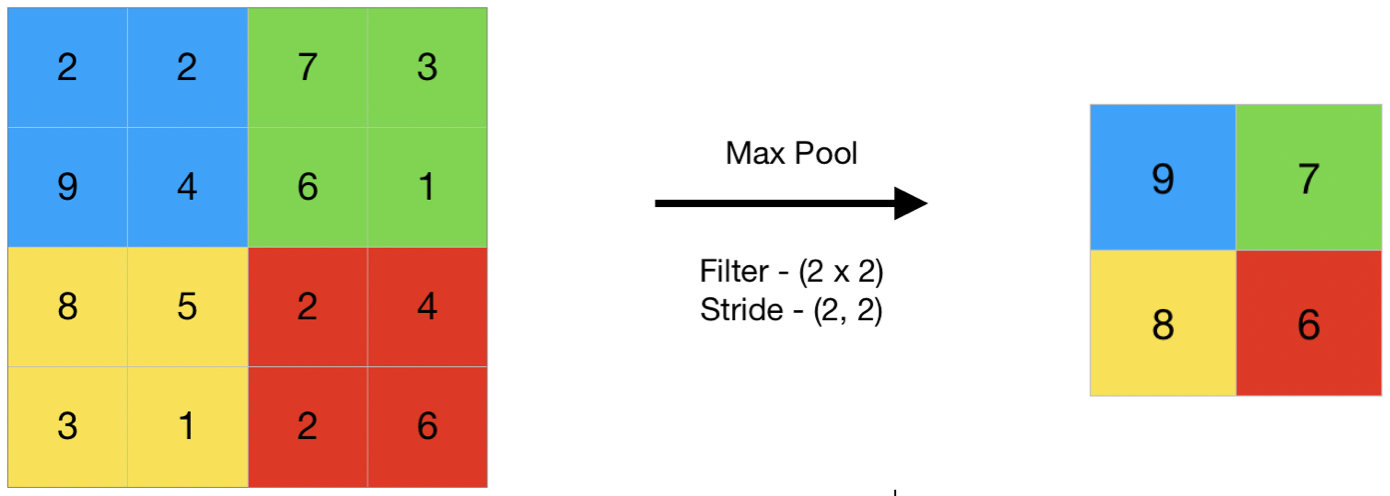
\includegraphics[width=0.75\linewidth]{Screenshot-2019-07-21-at-2.57.13-AM.png}
\caption{\label{fig:Pooling}MaxPooling}
\end{figure}

\subsection{Teljesen összekapcsolt réteg }

Teljesen kapcsolt réteg (Fully Connected, Dense, Linear Combination): előállítja a bemenetek és egy tárolt súlymátrix lineáris kombinációját: 
 $H=XW+b$, ahol X a bemeneti mátrix, W a súlymátrix, b egy opcionális eltolósúly-vektor.

\subsection{Batch normalizálás}

A batch normalizációs rétegek segítik a túltanulás megelőzését és normalizált batchek mellett megfigyelhető a háló tanulási sebességének javulása is, ugyanis a Neurális hálók az információt "kötegekben" vagyis batch-ekben dolgozzák fel, így ez a réteg egy köteg átlagát és szórását egységesen normalizálja az alábbi módon:

\noindent Átlag: $atlag = 1/m \displaystyle\sum_{i=1}^{m} x_i$  \newline
Szórás: $szoras = 1/m \displaystyle\sum_{i=1}^{m} (x_i – atlag)^2 $\newline
Normalizált aktivációk: $yi = (x_i – atlag) \sqrt(szoras + \epsilon)$ \newline
\newline
\textit{Átskálázott és eltolt aktivációk}:$ z_i = \gamma y_i + \beta $, 
\textit{ahol} $\gamma$ \textit{és} $\beta$  \textit{tanult paraméterek}
\newpage
\section{Yolov5 és gyakorlati alkalmazása}
\subsection{YOLOv5 és használt verziók}

A Yolo(You only look once) algoritmus egy Joseph Redmon, Santosh Divvala, Ross Girshick és Ali Farhadi által kitalált algoritmuson alapuló neurális háló amiből a félév során a Yolov5-öt (arhitektúra:\autoref{fig:architecture}) használtam amit az Ultralytics készített. A Yolo egy egészen új megközelítés a computer vision világában. Működés közben a képet rácsrendszerre osztja, és minden egyes rács a saját területén lévő objektumokat érzékeli. Innen is ered a név, egy lépésben végzi az objektumdetekciót és a lokalizációt is, tehát "Egyszer néz rá".
\par A háló tanító bemenetére elvárja a képet és egy txt szövegfájlt amiben a képen található objektumok találhatóak id, középpont, szélesség, és hosszúság, szerint.

\begin{figure}[ht]
    \centering
    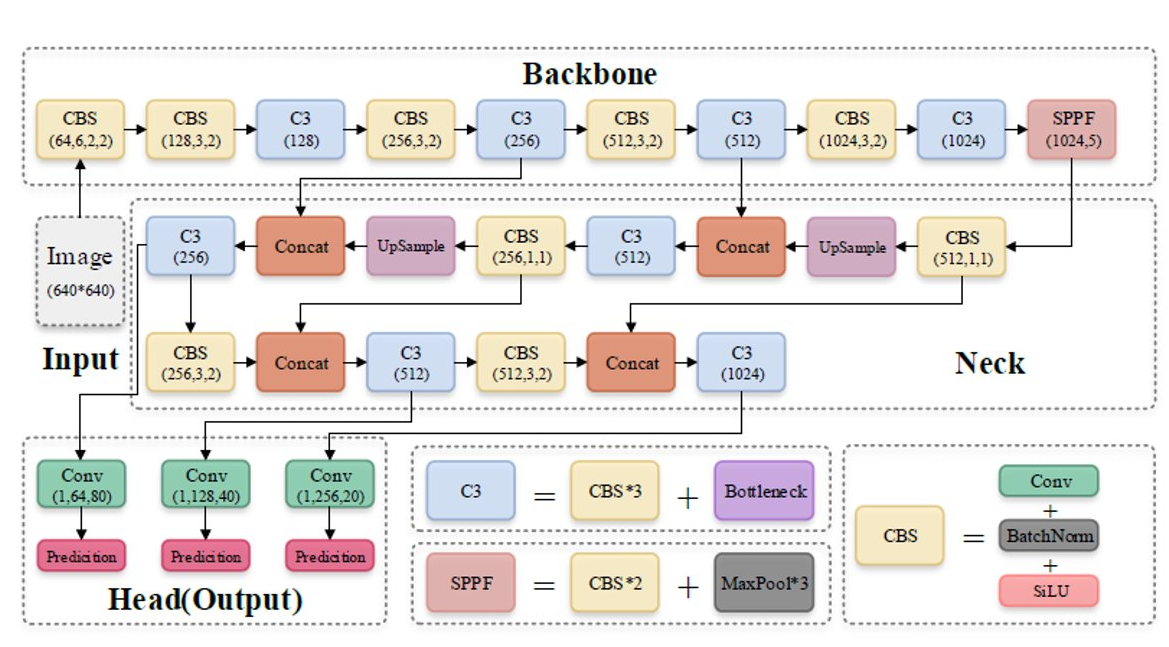
\includegraphics[width=1
    \linewidth]{architecture.png}
    \caption{\label{fig:architecture}Yolov5 architecture from Ultralytics github}
\end{figure}
\vspace{3mm}\par
\noindent A továbbiakban a Yolov5- öt használtam az Ultralytics github repository-jából töltöttem le: 
\vspace{1mm}\par
\noindent \href{https://github.com/ultralytics/yolov5}{https://github.com/ultralytics/yolov5}
\vspace{2mm}\par
\noindent A Yolov5 \cite{yolov5github} hálónak öt ismert verziója van, amik méretükben és így effektivitásukban térnek el egymástól:
\vspace{2mm}\par
\begin{enumerate}
\item Yolov5n (nano) ~1,9 millió paraméter,
\item Yolov5s (small) ~7,2 millió paraméter.
\item Yolov5m (medium) ~21,2 millió paraméter.
\item Yolov5l (large) ~46,5 millió paraméter.
\item Yolov5x (extra large) ~86,7 millió paraméter. \noindent\par
\end{enumerate}
\vspace{3mm}
\noindent Ezek közül hardveres megkötések miatt a Yolov5s-et választottam, ami bár alulteljesít a nagyobb hálóknak, de a céljainknak megfelel, \noindent
\noindent hiszen ez a háló bár előretanított a COCO adathalmazon ( ez egy sokosztályos adathalmaz, nem feltétlenül közlekedési objektumokra, 80 objektuma között állatok és hétköznapi tárgyak) rendelkezik egy valamilyen szintű kompetenciával a közlekedéi objektumok detektálására.

\newpage
\subsection{Adathalmaz, Cityscapes}
 Ezt a hálót tanítottam felül hogy az általam kitűzött cél elérésére, a közlekedési objektumok detektálására, erre használtam fel a "Cityscapes dataset"\cite{cityscapes}-et.\par 
 Hogy a hálónk effektívebb legyen csak 8 osztályt hagytam meg abból inkább 6 osztály észlelésére tanítottam felül,8 osztály az eredeti adathalmazból \textit{(gyalogos, autó, bicilkis, motoros, busz, vonat, kamion, ismeretlen)} de a Cityscapes-ben csak ebből 6 található\textit{(gyalogos, autó biciklis, motoros, busz, kamion)}, erre felültanítottam,
 a másik adathalmaz a \textbf{CityScapes} annak is a "\textit{gtfine}" nevű finoman annotált adatbázisával, aminek az osztályai, és a COCO adathalmaz osztályainak a metszete hat osztály (gyalogos, autó,biciklis, motoros, kamion, busz).A finom annotáció ebben a helyzetben azt jelenti hogy az objektumokat egymástól elszegmentálták és a 'corse' annotációhoz képest lényegesen több pontot használtak poligonok leírásához, amik a szegmentációs maszkokat írják le.Az adatbázis annotált és nyers képeket tartalmaz
 közúti/városi helyzetekről, több évszakban(tavasz, nyár, ősz), változó fényviszonyok között és különböző időjárási viszonyok között lett felvéve egy fedélzeti kamera (dashcam) szemszögéből.
 \par Az szegmentációs maszkokat minden képhez egy json fájl tárolja, ezekben az objektumok poligonokként, azok pontjaival vannak leírva (és a pontok x és y pozíciójukkal megadva, ezek esetén a mértékegységet a kép adott tengelyen való kiterjedésében adták meg), és egy el vannak látva egy id-vel ami az objektum osztályát hordozza információként.


\subsection{Formátumkonverzió}
Az előbbi bekezdésekből megérthettük hogy az adathalmaz és a háló bemenete nem ugyanazon a formátumon van (poligon $\neq$ bounding box),
ezért írni kellett egy átalakítót ami ezt az átalakítást, gyorsan és megbízhatóan elvégzi, erre egy egyszerű algoritmust írtam.
\newline
\begin{verbatim}
for v in "poligon pontjai": 

    maxx=max(v.x,maxx)      //négyzet legjobboldalibb pontja
    
    minx=min(v.x,minx)      //négyzet legbaloldalibb pontja
    
    maxy=max(v.y,maxy)      //négyzet legfelso pontja
    
    miny=min(v.y,miny)      //négyzet legalsó pontja
\end{verbatim}
Ezekből a pontokból csinálunk egy tégalalpot az alábbi módon:
A téglap középpontját úgy hatérozzuk meg hogy a 
\begin{verbatim}
for v in "poligon pontjai": 

    width=maxx-minx     //szélesség két szélso x koordináta különbsége
    
    height=maxy-miny    //magasság a két szélso y koordináta különbsége
    
    centerx=(maxx+minx)/2   //a középpont a két szélso 
    centery=(maxy+miny)/2   //koordinátapáros átlaga
    
\end{verbatim}

\subsection{Tanítás és validáció, adatok kiértékelése}
A Yolov5s modellt felültanítottam a már hálónak megfelelő formátumra, írtam egy gyors adathalmaz leíro '.yaml' kiterjesztésű fájlt az adathalmaz helyéről és megkezdtem a tanítást.

\begin{lstlisting}[language=bash]
$ python train.py --img 1024 --epochs 10 --data Traffic.yaml
        --weights yolov5s.pt --batch-size 4
\end{lstlisting}
Tehát a tanítást a yolov5s.pt-n végeztem 1024 pixeleses felbontáson, 10 epochon keresztül végeztem, és egyszerre a háló 4 képet kapott, ezt írja le a fenti parancs. 
A tanítás 13 órát vett igénybe és sikerrel zárult, a yolov5 háló elkészítette a validáció eredményeit bemutató infografikákat:
\autoref{fig:confusion}

\begin{figure} [ht]
    \centering
    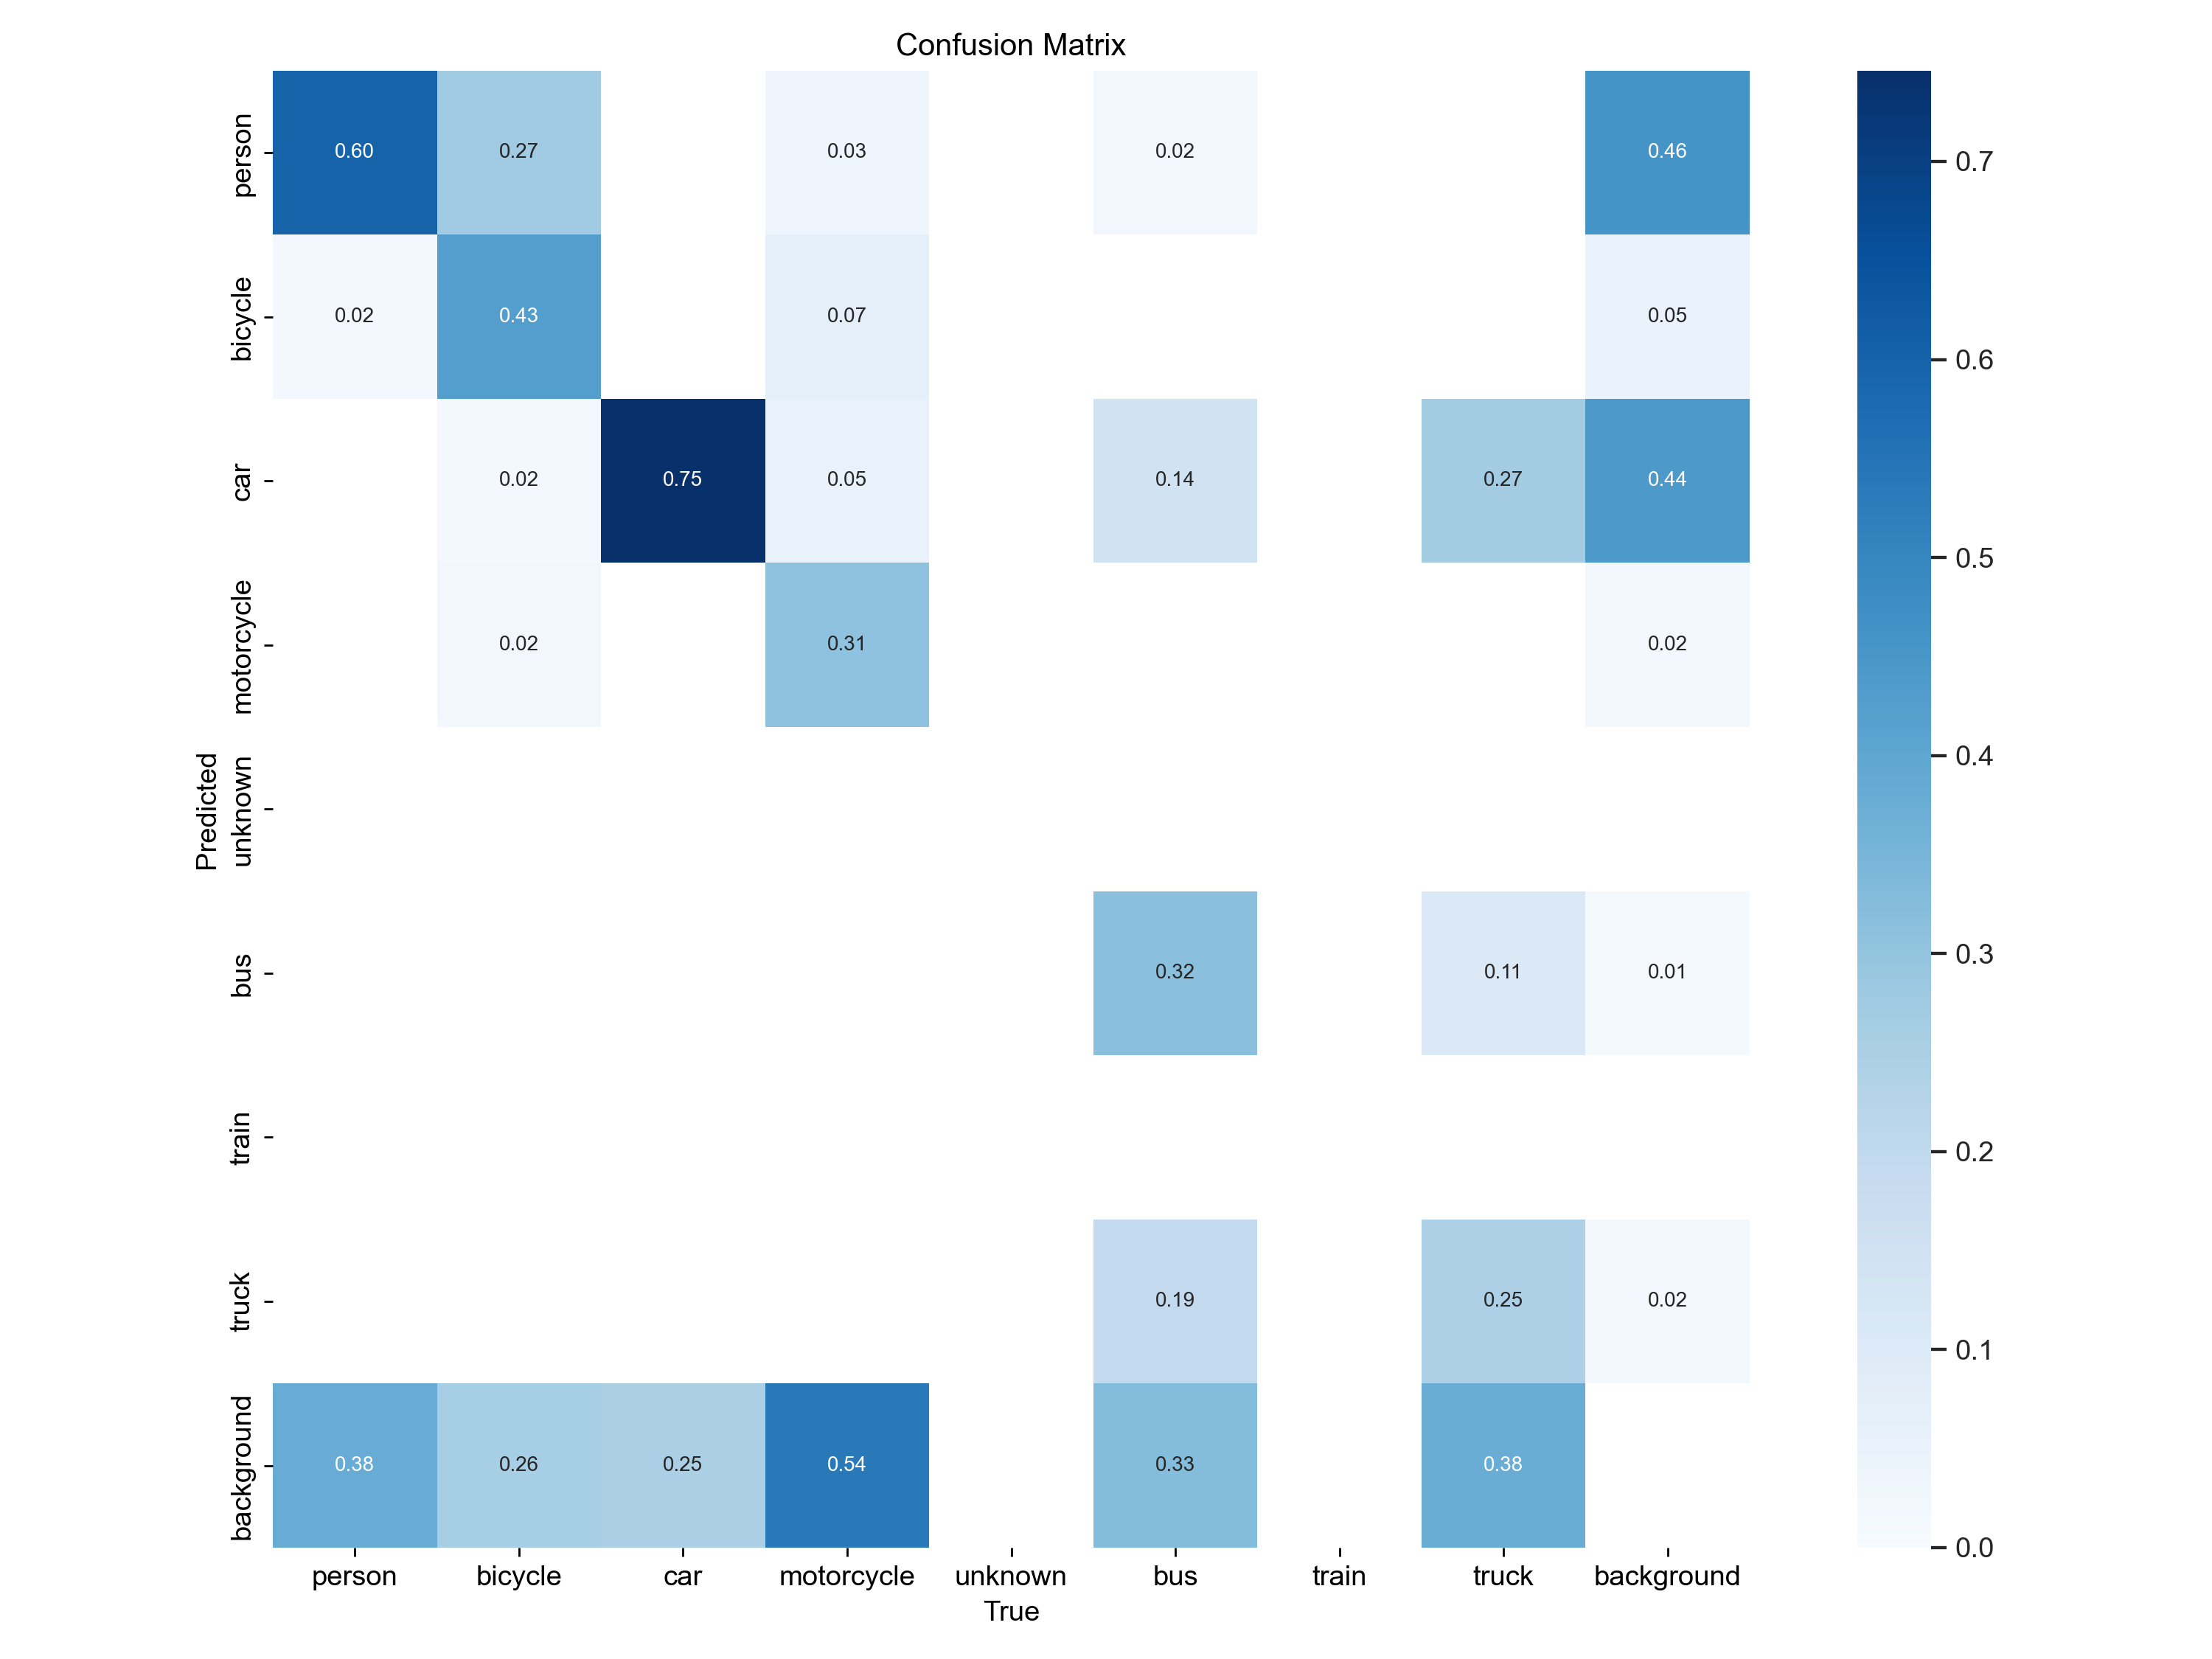
\includegraphics[width=1\linewidth]{confusion_matrix.png}
    \caption{Confusion matrix}
    \label{fig:confusion}
\end{figure}
\newpage
A confusion matrix kiértékelésekor azt tatláltam hogy az autókra is gyalogosokra kimondottan érzékeny a háló, ahhoz hogy ezt megértsük látnunk kell a tanító adathalmazt és azon belül azt hogy milyen a tanító adathalmaz osztályainak eloszlása. 
\par
Ahogy láthatjuk a gyalogosok és az autók túlnyomó többségben vannak így túlreprezentáltak és eltorzítják az érzékenységét a hálónak az irányukba.


\begin{figure}[hb!]
    \centering
    \includegraphics[width=0.55\linewidth]{labels.png}
    \caption{Labelek eloszlása}
    \label{fig:labels}
\end{figure}
\subsection{Megoldás}
A problémát az érzékenységi egyensúly megtalálása jelenti. Mivel a gyalogosok és autók túlnyomó többségben vannak, z YOLO háló érzékenyebbé válik rájuk. A megoldás lehet a tanító adathalmaz újraegyensúlyozása.

Az egyensúlyhiány kiküszöböléséhez több módszer is alkalmazható:

1. \textbf{Adatmódosítás}: Több képet kell beszerezni olyan osztályokról, amelyek alulreprezentáltak (például buszok), hogy a háló ne favorizálja a felülreprezentált osztályokat.

2. \textbf{Működési módok finomhangolása}: Finomhangolhatjuk a YOLO paramétereit, például az osztályok súlyait, a példák súlyozását és a veszteségfüggvény paramétereit.

3. \textbf{Nagyobb hálózat}: Nagyobb YOLO verziókra tanítás (pl. YOLOv5m, YOLOv5l, YOLOv5x), melyek több paraméterrel rendelkeznek és lehet, hogy jobb eredményeket érünk el használatukkal.


\listoffigures

\end{document}